\documentclass{jsarticle}

\usepackage{listings,jlisting}
\usepackage[dvipdfmx]{graphicx}
\usepackage{bmpsize}
\usepackage{bm}

\lstset{
    basicstyle={\ttfamily},
    identifierstyle={\small},
    commentstyle={\smallitshape},
    keywordstyle={\small\bfseries},
    ndkeywordstyle={\small},
    stringstyle={\small\ttfamily},
    frame={tb},
    breaklines=true,
    columns=[l]{fullflexible},
    numbers=left,
    xrightmargin=0zw,
    xleftmargin=3zw,
    numberstyle={\scriptsize},
    stepnumber=1,
    numbersep=1zw,
    lineskip=-0.5ex
}
\begin{document}

\title{計算機科学実験及演習4 エージェント 課題3}
\author{1029-28-2473 二見 颯}
\maketitle

\section{プログラム概要}
サポートベクター回帰を実装して、その性能を交差検証によって評価した。 \\
また、リスティングデータ(San Francisco)から民泊における価格の予測を行った。

\section{外部仕様}
\begin{itemize}
    \item dat\_main.py - dat データを SVR によって予測する
    \item sanfrancisco\_main.py - SanFrancisco データセットを扱い、GridSearch によるハイパーパラメータ最適化まで行う
    \item svr.py - SVR を実装する
    \item svr\_test.py - SVRegressor の回帰式を plot して確認する
    \item utils.py - load\_data, cross\_val\_regression を実装する 
    \item scaler.py - MinMaxScaler(正規化), StandardScaler(標準化)のクラスを実装
\end{itemize}

\section{内部仕様}

\section{評価結果}
\subsection{回帰式の確認}
sample10.dat, sample40.dat について、線形、非線形SVRで2次計画問題が正しく解けていることを確認したが、
その結果については省略する。 \\
1次元の説明変数による回帰を、実装した linear, 多項式カーネル, Gauss カーネル SVR および scikit-learn による Gauss カーネル SVR
に対して学習して、学習したものと同じデータを用いて予測した。 \\
http://scikit-learn.org/stable/auto\_examples/svm/plot\_svm\_regression.html\#sphx-glr-auto-examples-svm-plot-svm-regression-py
を参考にして、svr\_test.py を実装した。パラメータは以下の通り。
\begin{lstlisting}
svr_rbf = SVRegressor(ker_type='-g', p=1.0, c=1e3, eps=0.1)
svr_lin = SVRegressor(ker_type='-n', p=0.1, c=1e3, eps=0.1)
svr_poly = SVRegressor(ker_type='-p', p=2, c=1e3, eps=0.1)

# scikit-learn による SVR
svr_sk = SVR(kernel='rbf', gamma=1.0, C=1e3, epsilon=0.1)
\end{lstlisting}
\begin{figure}[!h]
\centering 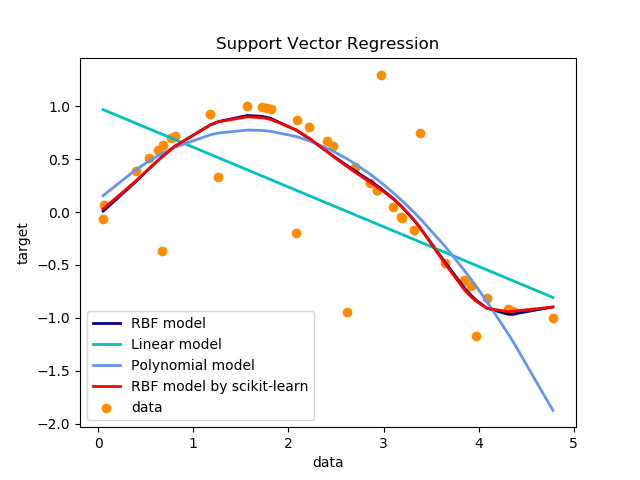
\includegraphics[width=15cm]{svr_verify.png}
\caption{verify SVR}
\end{figure}

\subsection{交差検証によるパラメータ探索(リスティングデータを用いる)}

\section{考察}
% SVR の式の意味(特に c, eps について)

% SanFrancisco data に関する考察


\section{参考資料}
\begin{itemize}
    \item scikit-learn と Tensorflow による実践機械学習 Aurelien Geron 著
\end{itemize}

\end{document}
